\exercisetitle{
Determinar la potencia disipada por la impedancia de carga $Z_L$ en el circuito de la figura, donde todas las líneas de transmisión son sin pérdidas $(Z_{01}= 50\Omega ,Z_{02}=Z_{03}= 70\Omega ,Z_S= 20 +j30\Omega,Z_L= 25 +j10Ω)$. Modifique convenientemente $l_2$ y $l_3$ para alcanzar, si es posible, máxima transferencia de potencia.
}

La estrategia a seguir para resolver este porblema será la siguiente:
\begin{enumerate}
  \item Sabiendo que para conseguir la máxima potencia de transferencia necesitamos que $Z_in = Z_S^*$ moveremos $Z_in$ $0.2\lambda$ hacia la carga.
  \item Escogeremos una $l_3$ tal que la parte real sea igual a la parte real de la $Z_in$ movida hasta dicho punto.
  \item Escogeremos $l_2$ de forma que la parte imaginaria de la admitancia de la suma de la sección $l_3$ más el stub sean igual a la encontrada en el primer paso.
\end{enumerate}

\begin{figure}[h]
  \centering
  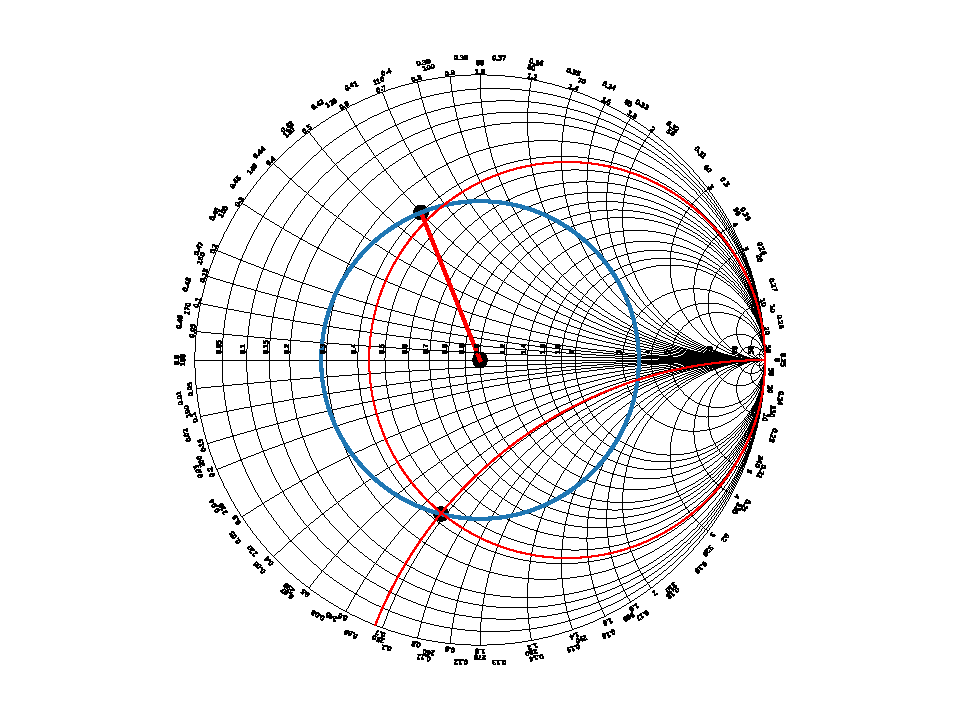
\includegraphics[scale = 0.75]{ej11/images/out1.pdf}
  \label{ej2smith}
\end{figure}
Obtenemos al final los valores normalizados $0.44 + 0.68j$ que al denormalizar y convertir en admitancia, obtendremos $y = 0.0134 -j0.02$

\subsection{$l_3$}
Para obtener la longitud $l_3$, nos moveremos por la línea, partiendo desde $y_l = 1/z_l= 2.62 -1.14 $, hasta encontrar una parte real de la admitancia igual a $0.0134$, que normalizado a la línea de $70 \Omega$ es $0.93$

\begin{figure}[h]
  \centering
  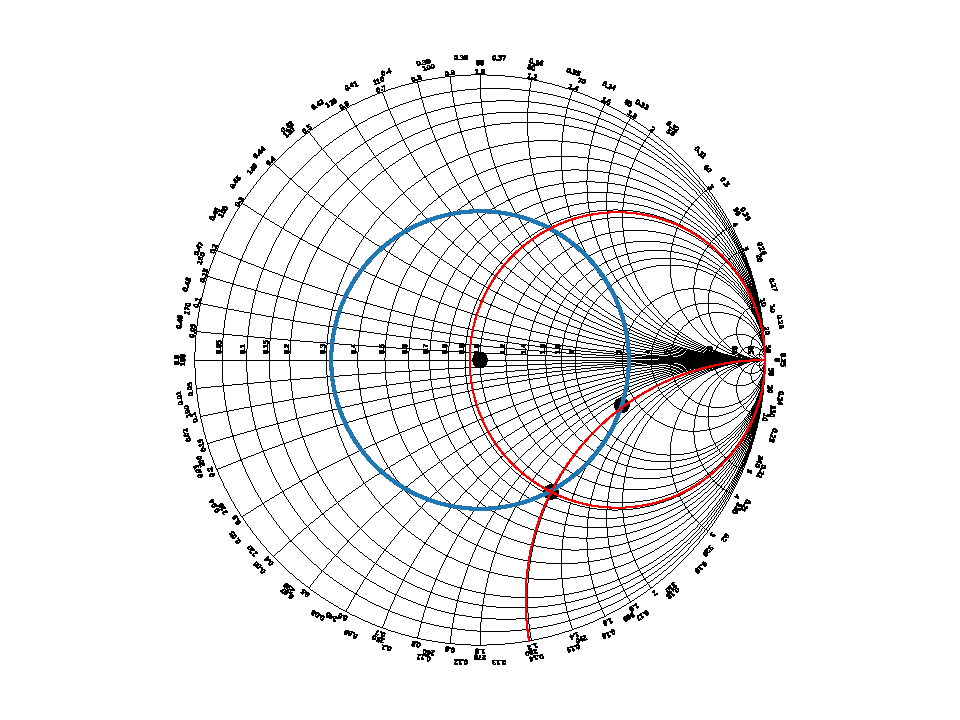
\includegraphics[scale = 0.75]{ej11/images/out2.pdf}
  \label{ej2smith}
\end{figure}

Donde vemos que esta la longitud de la línea ha de ser $0.1225\lambda$.

\subsection{$l_2$}
Como vemos la parte imaginaria de la admitancia de la línea $Z_L$ resultó ser -1.19, por lo que necesitamos un stub que nos situe la parte imaginaria en -0.02, por lo que de acuerdo con la ecuación (teniendo en cuenta que los valores estan normalizados):
\[y_{stub} = -j \frac{1}{tan{\beta l}} \]

Donde obtenemos $\beta l =   0.168$
